\documentclass{article}
%\usepackage{nips_2016}
\usepackage{iclr2018_conference, times}

%\usepackage[utf8]{inputenc} % allow utf-8 input
%\usepackage[T1]{fontenc}    % use 8-bit T1 fonts
\usepackage{hyperref}       % hyperlinks
\usepackage{url}            % simple URL typesetting
\usepackage{booktabs}       % professional-quality tables
\usepackage{amsfonts}       % blackboard math symbols
\usepackage{nicefrac}       % compact symbols for 1/2, etc.
\usepackage{microtype}      % microtypography
\usepackage{amsmath}
\usepackage{hyperref}
\usepackage{graphicx}

\definecolor{mydarkblue}{rgb}{0,0.08,0.45}
\hypersetup{colorlinks=true,
    linkcolor=mydarkblue,
    citecolor=mydarkblue,
    filecolor=mydarkblue,
    urlcolor=mydarkblue}

\newcommand{\vtheta}{\mathbf{\theta}}
\newcommand{\relaxed}{r}
\newcommand{\discreteDist}{p_{\theta}(b)}
\newcommand{\loss}{f(b)}
\newcommand{\lossGrad}{\loss{} \frac{\partial}{\partial \theta }\log \discreteDist{}}
\newcommand{\mcGrad}{\hat{g}}
\newcommand{\expectedLoss}{\mathbb{E}_{\discreteDist{}}[\loss{}]}
\newcommand{\expectedLossLogTrick}{\mathbb{E}_{\discreteDist{}}[\lossGrad{}]}
\newcommand{\var}{\text{Var}}



\title{Backpropagate through anything:\\ Reparameterization through learned control variates}

\author{
  David S.~Hippocampus\thanks{Use footnote for providing further
    information about author (webpage, alternative
    address)---\emph{not} for acknowledging funding agencies.} \\
  Department of Computer Science\\
  Cranberry-Lemon University\\
  Pittsburgh, PA 15213 \\
  \texttt{hippo@cs.cranberry-lemon.edu} \\
}

\begin{document}
\maketitle
\begin{abstract}
Gradient-based optimization is the foundation of deep learning and reinforcement learning.
Even when the mechanism being optimized is unknown or not differentiable, optimization using high-variance or biased gradient estimates is still often the best strategy.
We introduce a general framework for learning low-variance, unbiased gradient estimators for black-box functions.
These estimators can be jointly trained with model parameters or policies, and are applicable in both discrete and continuous settings.
We give unbiased, adaptive analogs of state of the art reinforcement learning methods such as deep deterministic policy gradients and advantage actor-critic.
We also demonstrate this framework for training discrete latent-variable models.
\end{abstract}



f is not optimal relaxation

concrete is not optimal relaxation

toy experiments

real exps on binary vae comparing:

%rebar

%g(z) (simple rebar)

%f(g(z))

%f(g_1(z)) + g_2(z)



\section{Introduction}
Gradient based optimization has been key to many recent advances in machine learning, the most notable of which being the use of deep neural networks as general purpose function approximators [cite SOME DEEP LEARNING STUFF].
Through the back-propagation algorithm [cite BACKPROP], the gradient of a loss function can be obtained with respect to each model parameter and learning can be accomplished via gradient decent.
Recent advancements such as Stochastic Variational Inference \cite{SVI} and the so-called "reparametization Trick" \cite{VAE} have enabled the use of gradient base learning for scalable, approximate inference enabling learning in vary large probabilistic models with complex approximating posterior ditributions [ cite NORMALIZING FLOWS OR SOMETHING].
Unfortunately, these approaches are limited to models with continuous random variables or very simple discrete structure. 

Discrete structure is prevalent in nature and can often much more efficiently represent the semantic information in high dimensional input so tractable approaches to learning in model with discrete latent variables is very appealing.
Unfortunately, training models with discrete random variables requires discontinuous sampling operations which keep us from utilizing low-variance reparameterization gradients explicitly.
Earlier approaches for dealing with this issue involve high-variance or biased gradient estimates, making learning slow and challenging for large probabilistic models.
The recently proposed REBAR estimator deals with this by combining the REINFORCE gradient estimator with a control variate based on a continuous relaxation of the discrete loss function which allows for unbiased and lower-variance gradient estimates.
The REBAR estimator also finds a functional form for the variance of the estimator which allows tuning of the estimator parameters via gradient decent to minimize the estimator variance. 

In this work, we study the assumptions made by the REBAR estimator and produce a new estimator, RELAX, which relaxes these assumptions by replacing the continuous relaxation from REBAR with a relaxation learned by a neural network to directly minimize the variance of the estimator.
We summarize our contributions below. 

The recently-developed REBAR method \citep{tucker2017rebar} reduces the variance of the REINFORCE gradient estimator by adding a control variate based on the concrete relaxation \citep{maddison2016concrete}.
The free parameters of REBAR can be tuned by gradient descent to minimize the variance of the estimator.
We generalize this method, showing that the particular relaxation used by REBAR is not necessarily optimal for minimizing variance. We present a new gradient estimator, RELAX, which replaces the REBAR's continuous relaxation with a neural network which is optimized during training. We validate this estimator on a number of generative modeling tasks, demonstrating improved performance over competing methods. 


[TODO: motivate necessity for this type of optimizing]

(check)gradient based optimization is dope af

(check)discrete latent structure is dope

(check)can?t fit because:

(check)discrete sampling keeps us from applying reparamaterization gradients 

(check)reinforce doesn?t get this info

(check)pay homage to rebar

introduces conditional reparam

(check)introduces gradient signal for minimizing variance




\paragraph{Contributions}
\begin{itemize}
\item we keep conditional reparam from rebar while exploring and expanding on gradient signal for minimizing variance of estimator
\item we generalize the concrete and muprop relaxations for a learnable family of functions that can be optimized via gradient decent to minimize the variance of the estimator
\item We show that concrete relax is not optimal, and that control variate based on the discrete objective at continuous input is is not the optimal control variate.
\item we combine these insights into a new family of estimators that generalizes rebar
\end{itemize}



\section{REINFORCE, Concrete, and REBAR gradient estimator}
% NOTE: this is a rough draft version of the final section
In this section we formalize the problem we are trying to solve and review important past work upon which we are building.

% problem formulation: simple stochastic system with discrete latent variable 
For simplicity of exposition, consider a simple stochastic model that has a discrete latent variable $b$ with probability $\discreteDist{}$ and loss function $\loss{}$.

Note we assume without loss of generality that $\loss{}$ is independent of the parameters  $\theta$ of $\discreteDist{}$.
Training the model involves minimizing the expected cost $\mathcal{L}(\theta)=\expectedLoss{}$.
This can be achieved efficiently using gradient optimization, requiring exact or approximate computation of $g=\partial\mathcal{L} / {\partial \theta}$.

In many cases of interest, an analytic form of the gradient $g$ is not known, and so an estimator $\mcGrad{}$ is required, such as the Monte Carlo estimator $\mcGrad{}\approx \sum_{i=1}^n\hat{g}(b_i) / n$ where $b_i\sim \discreteDist{}$ and $n$ is the number of samples. 

\subsection{REINFORCE}

% REINFORCE: baseline, doesn't work well without variance reduction

The REINFORCE gradient \cite{williams1992simple} expands $g$ as $\expectedLossLogTrick{}$ using the log-derivative trick \cite{LOG DERIVITIVE TRICK}, and uses exactly a Monte Carlo estimation scheme. 
However, the derivative of the log-likelihood w.r.t. its parameters (known as the score function in statistics) has high variance under Monte Carlo estimation, and so variance-reduction techniques such as control variates or Rao-Blackwellization are usually applied to improve the speed of convergence to a good solution.

\subsection{Concrete estimator}
% CONCRETE: relaxation, following level of detail in Tucker et al. 2017. Biased estimator.

Another approach to estimating the gradient of a loss that involves discrete random variables is a continuous relaxation. 
\cite{maddison2016concrete} and \cite{jang2016categorical} developed in parallel a reparameterization of a categorical distribution using the Gumbel-Max trick for sampling from a discrete distribution.

The reparameterization is intuitive to understand when considering each point in discrete distribution as one-hot vector.
Since we want the gradient to be defined at all points, we can extend the distribution over one-hot vectors to allow it to take values in its convex hull, so that the support is maintained of the discrete points in the support of the distribution.
The convex hull is the d-1 dimensional probability simplex in $\mathbb{R}^k$, where $k$ is the dimension of the discrete distribution.

Let $G_{1:k} = -\log-\log(U_{i:k})$ be samples from the Gumbel distribution, and learnable parameters $(\alpha_1, \dots, \alpha_k)$ be interpreted as some unnormalized parameterization of the discrete distribution under consideration.
Then, consider the following sampling procedure: for each k, find the k that maximizes $\log \alpha_k - G_k$, and then set $D_k=1$ and $D_{i \neq k} = 0$. The Gumbel-Max trick states that sampling from the discrete distribution is equivalent to taking this argmax, that is, $p(D_k = 1) = \alpha_k / \sum_{i=1}^n \alpha_i$.

Since taking an argmax is still a discontinuous operation, \cite{maddison2016concrete} and \cite{jang2016categorical} proposed further relaxing the argmax operator through the softmax function with an additional temperature parameter $\lambda$:
\begin{equation}
x_k = \frac{\exp\{( \log \alpha_k+ G_k) / \lambda\}}{\sum_{i=1}^n\exp\{( \log \alpha_i+ G_i) / \lambda\}}
\end{equation}
This relaxation allows values within the simplex, but in the low temperature limit, it becomes exactly the discrete argmax.
One limitation of the concrete distribution is that it is a biased estimator except in limiting temperature.
In other words, a small amount of bias is present for a non-zero temperature.

%** Note for next revision: tie this into the REBAR estimator by using the Logistic random variable used by \cite{tucker2017rebar} from the appendix of \cite{maddison2016concrete}.

%** Other points: Concrete trades lower variance for a biased estimator

\subsection{REBAR estimator}
% REBAR: unbiased estimator that combines REINFORCE with CONCRETE.

The REBAR gradient estimator develops a lower-variance gradient estimator that outperforms one based on a Concrete relaxation. REBAR relies on a carefully designed control variate, so we begin with a review of this theory.

\subsubsection{Control Variates for Variance Reduction}
For an unbiased estimator $f(b)$, a control variate is a function $\tilde{f}$ with a known or estimatable mean $\mathbb{E}[\tilde{f}]$. Since the mean of the function can be subtracted from the expectation, $f(b) - \eta (\tilde{f}-\mathbb{E}[\tilde{f}])$ remains an unbiased estimator.
A control variate is scaled by a constant $\eta$.
Note that we can write $\text{Var}(f(b)+\eta(\tilde{f}-\mathbb{E}[\tilde{f}]))$ as
\begin{align}
    \text{Var}(f(b)+\eta \tilde{f}) = \text{Var}(X) + \eta^2\var(\tilde{f}) + 2 \eta \text{Cov}(f(b),\tilde{f}),
\end{align}
which, evaluating the first derivative w.r.t. $\eta$ and solving for zero yields:
\begin{align}
    \eta = -\frac{Cov(f(b), \tilde{f})}{Var(\tilde{f})}.
\end{align}
The variance reduction effect of a control variate is induced by the high correlation of the control variate with the original estimator.
The intuition behind this is as follows.
When $f(b)$ and $\tilde{f}$ are positively correlated, then this means $\tilde(f)$ is large when $f(b)$ is large.
So, if in some minibatch $\tilde{f}$ is greater than its known mean, then with high probability $f(b)$ is also greater than its true mean.
That means this minibatch would contribute variance to the overall estimation algorithm, since the values we're estimating of $f(b)$ are with high probability greater than the true mean (the true gradient, in the case of REBAR). 
With positive correlation, $\text{Cov}(f(b), \tilde{f})) > 0$, and so $\eta$ is negative. 
Then, the effect of the control variate in such a minibatch is to reduce the REINFORCE estimate by subtracting the quantity $\eta(\tilde{f} - \mathbb{E}[\tilde{f}]$.

Hence, a suitably scaled control variate with high correlation to the original estimator dampens or amplifies the value of the overall estimator towards the true mean per minibatch.
The same explanation applies to the case where the correlation is negative by swapping the terms "lesser" for "greater" and "reducing" by "increasing".
This is why high correlation of $f(b)$ with $\tilde{f}$ is desirable: it renders the control variate effective in drawing down the effect of high variability in a stochastic estimator by a magnitude commensurate with the difference of a highly correlated function and its known mean.

\subsubsection{Reducing Gradient Variance through a Low-Variance Control Variate}
Following \cite{tucker2017rebar}, the following overview focuses on a single discrete Bernoulli random variable.
The core of the REBAR estimator is a REINFORCE-style estimate of a non-differentiable reparameterization of the discrete latent variable as $b=H(z)$, where $H$ is the hard-threshold function an
\begin{align}
z := g(u, \theta) := \log\frac{\theta}{1-\theta} + \log\frac{u}{1-u}, u \sim \text{Unif}[0,1]
\end{align}
While $z$ is a reparameterization that renders the parameters of $b$ learnable by gradient-based methods, $H$ introduces a new discontinuity in the loss.
Instead of relaxing the hard threshold as in \cite{maddison2016concrete}, \cite{tucker2017rebar} uses a REINFORCE estimator for the gradient reparameterized with $H(z)$:
\begin{align}
    \frac{\partial}{\partial \theta} \mathbb{E}_{p(b)}[f(b)] = \frac{\partial}{\partial \theta} \mathbb{E}_{p(u)}[f(H(z))] = \mathbb{E}_{p(u)}[f(H(z))\frac{\partial}{\partial \theta}\log p(z)]
\end{align}
This allows the parameters $\theta$ to be learned using gradient information, but the loss is still non-differentiable due to the hard threshold.
Since this uses a REINFORCE estimator, it also has high variance.

Hence, \cite{tucker2017rebar} develop a control variate. A natural continuous relaxation of the hard threshold function is the sigmoid function, leading \cite{tucker2017rebar} to choose a $H(z) \approx \sigma_\lambda(z) := \sigma(z / \lambda) = (1+\exp( - z / \lambda))^{-1}$.
This relaxation leads to the following control variate summed with its expectation:
\begin{align}
    \frac{\partial}{\partial \theta} \mathbb{E}_{p(z)}[f(\sigma_\lambda(z))] =  \mathbb{E}_{p(z)}[f(\sigma_\lambda(z))\frac{\partial}{\partial \theta}\log p(z)].
\end{align}
Unfortunately, simply applying this control variate was found to be ineffective. 
The author's key insight was to derive a low-variance form of this control variate that takes advantage of a conditional marginalization of the reparameterized $z$ given a particular choice of discrete $b$.
This introduces a second reparameterization $\tilde{z}$ of $p(z|b)$, which depends on another sample $v\sim \text{Unif}[0,1]$.
See \cite{tucker2017rebar} for details of the derivation.


The control variate has the following form:
\begin{align}
    f(\sigma_\lambda(\tilde{z}))\frac{\partial}{\partial \theta}\log p(H(z))
\end{align}
and noting that 
\begin{align}  \mathbb{E}_{p(u,v)}[f(\sigma_\lambda(\tilde{z}))\frac{\partial}{\partial \theta}\log p(H(z))] = \mathbb{E}_{p(u,v)}[\frac{\partial}{\partial \theta}f(\sigma_\lambda(\tilde{z}))  - \frac{\partial}{\partial \theta} f(\sigma_\lambda(z))]
\end{align}
gives us the REBAR gradient estimator: \begin{align}
    \frac{\partial}{\partial \theta} \mathbb{E}_{p(b)}[f(b)] = \mathbb{E}_{p(u,v)}[f(\sigma_\lambda(\tilde{z}))\frac{\partial}{\partial \theta}\log p(H(z))  - \eta f(\sigma_\lambda(\tilde{z}))\frac{\partial}{\partial \theta}\log p(H(z)) + \eta\frac{\partial}{\partial \theta} f(\sigma_\lambda(z)) - \eta\frac{\partial}{\partial \theta}f(\sigma_\lambda(\tilde{z})) ]
\end{align} where $\eta$ is trained to minimize the variance of the estimator. 

% ** TODO: place \eta in this equation?
The special form of $\tilde{z}$ yields a lower-variance gradient estimate because a number of the random variables are conditionally marginalized out of the estimator.
Two features of this control variate make it particularly effective: its high correlation with the REINFORCE gradient, and a low-variance, reparameterized form of certain terms in the estimator.

\section{RELAX: The generalized REBAR estimator}
The REBAR estimator uses a control variate that evaluates the original loss function at relaxed inputs, reparameterized both unconditionally (denoted $z$, and conditionally, denoted $\tilde{z}$).
The central result of this paper is that learning the function in the control variate leads to even better convergence properties.
Specifically, we generalize the conditional marginalization and control variate of REBAR to the following form:
\begin{align}
    \mathbb{E}_{p(u,v)}[\relaxed (\tilde{z};\phi)\frac{\partial}{\partial \theta}\log p(H(z))] = \mathbb{E}_{p(u,v)}[\frac{\partial}{\partial \theta} \relaxed(\tilde{z};\phi) - \frac{\partial}{\partial \theta} \relaxed(z; \phi)],
\end{align}
where \relaxed{} is a neural network with parameters $\phi$.

The generalized REBAR estimator replaces the loss function evaluations in the control variate with an adaptive $\relaxed$ function which is trained via gradient decent to minimize the variance of the estimator. As shown in \cite{tucker2017rebar}, this can be easily computed. Denoting the RELAX estimator as $r(\phi)$ we obtain:
\begin{align}
    \frac{\partial}{\partial\phi}\var{(r(\phi))} = \frac{\partial}{\partial\phi}\mathbb{E}[r(\phi)^2] + \frac{\partial}{\partial\phi}\mathbb{E}[r(\phi)]^2 = \frac{\partial}{\partial\phi}\mathbb{E}[r(\phi)^2] = \mathbb{E}[\frac{\partial}{\partial\phi}r(\phi)^2]
\end{align}
Where the second equality comes from the fact that for all $\phi$, the RELAX estimator is unbiased and therefore $\frac{\partial}{\partial\phi}\mathbb{E}[r(\phi)]^2 = 0$.

% This small change to the REBAR control variate yields a 
% dramatic % lets make sure we have the data to back that up
% reduction in variance on the same benchmark tests used by \cite{tucker2017rebar}.

% I think this section should go next
%\section{Properties of Optimal Relaxations}
% maybe we should change the name of this section to "Questioning the Concrete Relaxation" in which case maybe  it should go before the above section???
In \cite{tucker2017rebar} the concrete distribution \cite{maddison2016concrete} is used in the control variate due to its similarity to the Bernoulli distribution and assumed correlation with the target function (**TODO EXPAND THIS).

NEXT: PROVE THAT CONCRETE IS NOT THE OPTIMAL RELAXATION TO USE (SHOULD BE EASY TO PROVE BUT WE NEED TO DO IT)


%Using variational calculus, we can examine the form of the optimal relaxation $\relaxed{}$

Relaxing Assumptions

identifying assumptions other estimators in the past made

demonstrate (proof?) that those assumptions are not optimal

and that the optimum is a function of {f, theta}



\section{Experiments}
We demonstrate the effectiveness of our estimator on a number of challenging optimization problems. Following \cite{tucker2017rebar} we begin with a simple toy example to illuminate the potential of our method and then continue to the more relevant problems of optimize binary VAE's and reinforcement learning (OR GRAPH STRUCTURE LEARNING).


NEXT: OPTIMAL RELAXATION FOR TOY PROBLEM
NEXT: ELABORATE ON DEPENDENCE ON THETA


**TODO NEW EXPERIMENT: HALFWAY THROUGH A VAE TRAINING STOP, AND OPTIMIZE THE VARINACE OF \relaxed{} AND OF REBAR WRT TEMP AND ETA AND COMPARE GRADIENTS

\subsection{Toy Experiment}
We seek to minimize $\mathbb{E}_{b \sim p(b|\theta)}[(b - t)^2]$ as a function of the parameter $\theta$ where $p(b|\theta) = \mathtt{Bern}(b|\theta)$. \cite{tucker2017rebar} set the target $t = .45$. Here, we focus on the more challenging case where $t = .499$. With this setting of the target, REBAR and competing methods suffer from high variance and are unable to discover the true solution of $\theta = 0$.

The fixed Concrete relaxation of REBAR is unable to produce a gradient who's signal outweighs the sample noise and is therefore unable to solve this problem noticeably faster than REINFORCE. Figure \ref{fig:toy_var} plots the learned relaxations for a fixed value of $\theta$. It can be seen that RELAX learns a relaxation who's derivative points in the direction of decreased loss for all values of reparameterization noise $u$ whereas REBAR's fixed relaxation  only does for values of $u > t$. (NEED TO VERIFY THIS IS RIGHT)

[pictures, variances graphs]
\begin{figure}
\begin{center}
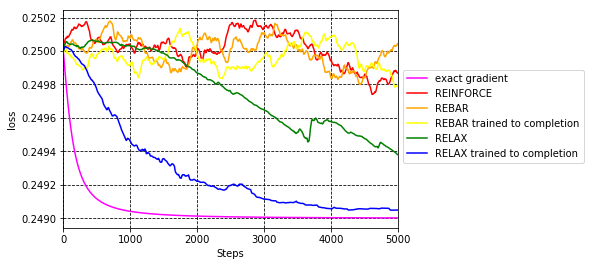
\includegraphics[scale=.33]{figures/losses}
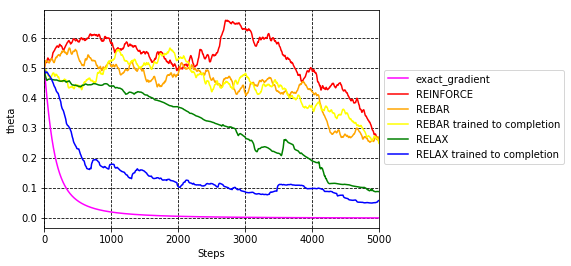
\includegraphics[scale=.33]{figures/theta}
\end{center}
\label{fig:toy_loss}
\caption{Estimator loss (left) and estimated $\theta$ values (right). Estimators with fixed (or no relaxation) struggle to converge to the optimal value}
\end{figure}

\begin{figure}
\begin{center}
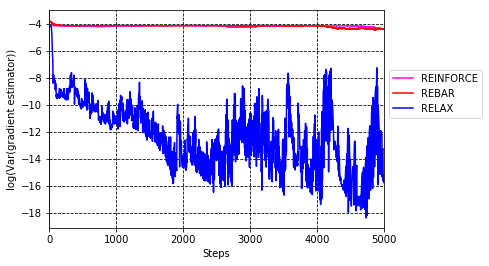
\includegraphics[scale=.33]{figures/variance_no_opt}
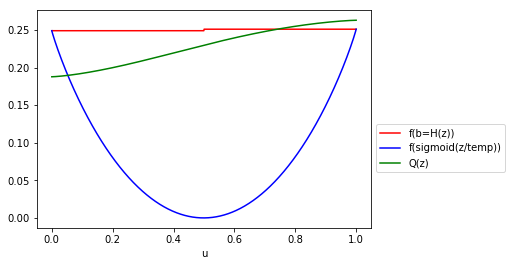
\includegraphics[scale=.33]{figures/learned_r}
\label{fig:toy_var}
\end{center}
\caption{Left: Estimator variance. Right: Learned relaxation function for fixed $\theta$}
\end{figure}
[head to head comparisons] 

\subsection{Discrete Variational Autoencoder}
As in \citep{tucker2017rebar}, we benchmark the RELAX estimator on the task of training a variational autoencoder \cite{VAE} where all random variables are Bernoulli taking values in $\{-1, 1\}$. As in \cite{tucker2017rebar}, we compare training the variational lower-bound across the MNIST \cite{MNIST} and Omniglot \cite{OMNIGLOT} datasets. As in \cite{tucker2017rebar} we test models with 1 and 2 of Bernoulli random variables with linear mappings between them and a model with 1 layer of Bernoulli random variables with non-linear mappings between layers.

We found that due to the complicated structure of the loss function, the RELAX estimator performed worse than REBAR. Instead we add a learned relaxation to REBAR's control variate which we denote relaxed-REBAR. Our estimator takes the form of \ref{eq:RELAX} with $$\bar \relaxed(z) = \relaxed(z) + f(\sigma_\lambda(z))$$ where $\relaxed(z)$ is a learned neural network and $f(\sigma_\lambda(z))$ is the Concrete relaxation of REBAR with temperature parameter $\lambda$. In all experiments, adding the learned $\relaxed(z)$ reduced the variance of the gradients and improved the final results. 

In \citep{tucker2017rebar}, a separate REBAR estimator was used to estimate the gradients of each model parameter (each weight matrix and bias vector). To apply our estimator to this formulation, we would need to learn a separate relaxation for each model parameter. To get around this, we instead place one gradient estimator on each activation that parameterizes a layer of Bernoulli variables. We then back-propagate this gradient estimate to produce a gradient estimate for each model parameter. To provide a fair comparison, we re-implemented REBAR in this way (denoted REBAR-ours in table \ref{tab:vae}). We believe this explains the large difference in performance between our implementation and that of \citep{tucker2017rebar} for the nonlinear models since there are 3 layers of parameters that all share the same gradient estimator. In the linear models, each layer has its own gradient estimator making our implementation closer to that of \citep{tucker2017rebar}.



[VAE, results, variances]
\begin{figure}
\begin{center}
 \begin{tabular}{|c|c c c||} 
 \hline
 \textbf{MNIST gen.} & REBAR \citep{tucker2017rebar} & REBAR-ours & relaxed-REBAR \\ [0.5ex] 
 \hline
 Linear 1 layer   & -111.6 & -111.66 & \textbf{-111.22} \\ 
 Linear 2 Layer & -98.8  & -98.23 & \textbf{-98.04} \\
 Nonlinear         & -101.1  &  -83.02 &  \textbf{-79.49} \\
 \hline\hline
 \textbf{Omniglot gen.} &&&\\
 \hline
 Linear 1 layer   & -116.83  & -116.75 & \textbf{-116.62} \\ 
 Linear 2 Layer & -108.99  & -108.74 & \textbf{-108.63} \\
 Nonlinear         & -108.72  & -62.28 & \textbf{-60.32} \\
 \hline
\end{tabular}
\end{center}
\label{tab:vae}
\caption{Training variational lower bound after training.}
\end{figure}


\subsection{Atari}

\citet{mnih-dqn-2015}


\section{Related Work}
\label{related work}

NVIL, VIMCO, things like that

\par{Generalized Reparameterization Gradients}
REBAR and the generalization in this paper uses a mixture of score function and reparameterization gradients.
A recent paper by \cite{ruiz2016generalized} unifies these two gradient estimators as the generalized reparameterization gradient (GRG).
This framework can help disentangle the various components of generalized REBAR.

REBAR innovation as further decomposition the correction term into secondary reparameterization components
note this is a recursive application of the principles of GRG
observe that the GRG suggests this recursive application to components of an estimator
propose that other estimators could be similarly recursively decomposed?


[TODO: cite certigrad arxiv 1706.08605]



\section{Limitations}
\label{limitation}

\section{Conclusion}
\label{conclusion}


\bibliography{bibliography}
\bibliographystyle{iclr2018_conference}


\section{Appendix A: Control Variates}
% basic definitions following level of detail in Tucker 2017


%\section{Understanding the REBAR estimator through the Generalized Reparameterization Gradient}

% ** Questions to answer: 
% (1) is z-tilde a clever way of using Rao-Blackwellization for a part of the reparameterization gradient? This would mean that the reparameterization z-tilde is related to the sufficient statistic of the estimator...
% (1) also maybe: the Q function has the opportunity to learn an estimator based on the sufficient statistics of the model, which by Rao-Blackwell-Kolmogorov is lower variance
% (2) What's a better notation to keep the dependence of z on $\theta$ in view?
% (3) is the REBAR control variate really using the reparameterization gradient in a meaningful way? Or, is it best viewed as just another f + control variate where control variate is cleverly designed with lower variance? 



%\subsection{Combining score function and reparameterization gradients}

\par{Generalizing the reparameterization trick}

Write sample from distribution $s(\epsilon)$ as $\epsilon = \mathcal{T}^{-1}(\mathbf{z}; \mathbf{\nu})$ for some invertible transform $\mathcal{T}$ with variational parameters $\nu$.
write out transformed density
example: normal with standard normal $s$
example: inverse CDF of Gaussian with uniform $s$
write out expected gradient under transformation
show decomposition of expected gradient into reparameterization and correction terms 

%\par{Applying GRG to REBAR}

%show mapping of terms
%note denser derivation in REBAR appendix

%\par{Interpreting REBAR through GRG}








\end{document}
